\begin{refsection}
    \renewcommand{\thefigure}{\arabic{figure}}
    
    \chapterTwoLines
    {Matemática na arte}
    {Uma proposta interdisciplinar para o ensino de geometria}
    \label{chap:matematicanaarte}
    
    \articleAuthor
    {Charles Ricardo Lemos de Melo}
    {Graduado em Matemática pela Universidade Federal do Rio Grande do Norte (UFRN). Graduação em Engenharia Civil pela UFRN. Especialista em Avaliação e Perícia de Engenharia pelo Centro de Pós-Graduação, Pesquisa e Difusão Cultural das faculdades Oswaldo Cruz. Professor da rede estadual do RN. E-mail: charlesrlemos@hotmail.com.}
    
    \articleAuthor
    {Wguineuma Pereira Avelino Cardoso}
    {Graduada em Matemática pela Universidade Federal do Rio Grande do Norte (UFRN). Graduação em Pedagogia pela UFRN. Especialização na área da Matemática para o Ensino Fundamental e Ensino Médio pelo Instituto Superior de Educação Presidente Kennedy. Mestrado na área de Ensino e Ciências pela UFRN. Doutoranda em Ensino de Ciências e Matemática pelo PPGECM (UFRN). ID Lattes: 3384.1278.8608.5225. ORCID: 0000-0002-5587-5766. E-mail: wguineuma@ifesp.edu.br.}
    
    \begin{galoResumo}
        \marginpar{
            \begin{flushleft}
            \tiny \sffamily
            Como referenciar?\\\fullcite{SelfMeloAndCardoso2021Matemática}\mybibexclude{SelfMeloAndCardoso2021Matemática}, p. \pageref{chap:matematicanaarte}--\pageref{chap:matematicanaarteend}, \journalPubDate{}
            \end{flushleft}
        }
        Este artigo aborda uma pesquisa que teve como objetivo investigar como a Arte pode contribuir no ensino e aprendizagem da Geometria. Elaboramos uma proposta interdisciplinar de ensino que utiliza imagens de telas de pintura a óleo como veículo de investigação dos elementos geométricos presentes nestas. Utilizamos telas de autoria do professor investigador da pesquisa e algumas composições dos artistas Mondrian e Kandinsky. A pesquisa experimental foi desenvolvida em uma escola pública, com alunos do 6º ano do Ensino Fundamental. Verificamos uma maior participação por parte dos alunos em sala e, ainda, uma atitude mais reflexiva e significativa, durante as discussões referentes aos conteúdos geométricos. 
    \end{galoResumo}
    
    \galoPalavrasChave{Artes Visuais. Formas Geométricas. Ensino.}
    
    \begin{otherlanguage}{english}
    
    \fakeChapterTwoLines
    {Mathematics in art}
    {An interdisciplinary proposal for geometry teaching}
    
    \begin{galoResumo}[Abstract]
        This article addresses a research that aimed to investigate how Art can contribute to the teaching and learning of Geometry. We developed an interdisciplinary teaching proposal that uses images from oil painting canvases as a vehicle for investigating the geometric elements present in them. We used canvases authored by the research professor and some compositions by artists Mondrian and Kandinsky. The experimental research was carried out in a public school, with students from the 6th year of elementary school. We verified a greater participation by the students in the classroom and, also, a more reflective and significant attitude during the discussions regarding geometric contents. 
    \end{galoResumo}
    
    \galoPalavrasChave[Keywords]{Visual arts. Geometric shapes. Teaching.}
    \end{otherlanguage}

    \section{Introdução}

    O ser humano está inserido em um mundo cercado de formas, sejam elas regulares ou irregulares, e é na Geometria que está organizada o conhecimento para entender esse espaço físico cercado de modelos geométricos no qual vivemos. Por isso, nos motivamos como docente, a tentar estimular o aluno a apropriar-se dos conhecimentos advindos da Geometria de modo a propiciar o seu desenvolvimento cognitivo na área da Matemática além de contribuir para obtenção de uma efetiva relação dessa área do conhecimento com o mundo que o cerca. 

    Em nossa prática docente, na disciplina de Matemática, com estudantes do Ensino Fundamental e do Ensino Médio, pudemos observar por diversas vezes, que os alunos podem apresentar algumas dificuldades em aprender Geometria. E essas dificuldades muitas vezes advêm de dois fatores: O primeiro é que uma boa parte dos professores privam os alunos da aprendizagem de Geometria, na medida em que selecionam os conteúdos que serão estudados em sala de aula. O outro fator a ser considerado, diz respeito a forma que alguns discentes ministram os conceitos geométricos em sala. Sobre isso alguns autores enfatizam que: 

    \begin{quotation}
        Os conceitos são ideias a serem construídas pelo aluno. Esta construção exige o trabalho de mediadores (professores, colegas materiais instrucionais, entre outros) que contribuam para atribuições de significado aos fenômenos estudados, no caso associados às formas, ao espaço ou suas representações. \cite[p.~7]{RÊGOAndRÊGOAndKLEBER2012Laboratório}.
    \end{quotation}

    Assim, é necessário que os conteúdos geométricos sejam apresentados de uma forma mais significativa para os estudantes, uma sugestão seria associar a Geometria a outras áreas de conhecimento. 

    Utilizando como pressuposto que o ensino da Matemática tenha uma relevância considerável para o processo de formação social e cultural dos indivíduos, a presente pesquisa tem como intuito buscar outras formas de ensino e aprendizagem da Matemática aliada a outras áreas do conhecimento, de modo que seja proporcionado aos alunos um aprendizado que o estimule a raciocinar sobre a Geometria presente no seu cotidiano.  

    Diante disso, temos vários questionamentos vivenciados em nossa prática: De que forma poderíamos associar a Matemática do cotidiano aos nossos alunos? O que fazer para apresentar o conteúdo de Geometria, em especial, o estudo das principais figuras planas de uma forma prazerosa, amena e interessante, sem que se perdesse de vista o seu rigor, no que diz respeito aos conceitos matemáticos? Como utilizar outras áreas do conhecimento no ensino de Matemática? 

    A partir do que foi posto, propomos agregar o ensino da Geometria, no que diz respeito aos conceitos de figuras planas, à Arte e, no caso particular a pintura, tentando integrá-los, de um modo harmonioso e atrativo para os discentes, além de oportunizar a inserção de elementos artísticos ao longo do processo, propiciando uma conexão da disciplina de Matemática com a Arte, em especial às Artes Visuais, de modo a contribuir para uma efetiva apropriação, pelos alunos, dos conceitos geométricos apresentados em sala, além de tornar as aulas de Geometria mais dinâmicas imbricadas de significados. 

    Assim, nosso objetivo é investigar como a Arte pode contribuir no processo ensino-aprendizagem da Geometria em duas turmas do 6º Ano do Ensino Fundamental. Além disso, buscamos identificar as potencialidades e limitações no ensino de Geometria aliado à Arte; elaboramos e aplicamos algumas atividades didáticas, e por fim planejamos e desenvolvemos aulas, em uma escola pública do Rio grande do Norte (RN), nas quais utilizamos a Arte como caminho para o ensino e aprendizagem de Geometria. E, uma de nossas referências para essa investigação foi à interdisciplinaridade de \textcite{FAZENDA2011Integração}, que tem como princípio reconhecer as limitações nas aprendizagens fragmentadas \cite{FAZENDA2011Integração}. E depois, por meio dos experimentos e das atividades realizadas, fizemos nossas observações de campo, que segundo, \textcite{LAVILLEAndDIONES1999Construção}:  

    \begin{quotation}
        [\dots] revela-se certamente nosso privilegiado modo de contato com o real: e observando que nos situamos, orientamos nossos deslocamentos, reconhecemos as pessoas, emitimos juízos sobre elas. Sem alongar inutilmente essa lista, convenhamos que, em nossas atividades quotidianas, não há quase exemplos que não deixem espaço a observação \textcite[p.~177]{LAVILLEAndDIONES1999Construção}. 
    \end{quotation}

    Dessa forma, a observação das experiências desenvolvidas em campo, permitiu um olhar para nosso objeto de pesquisa. Assim, descrevemos nossas observações neste artigo que está dividido em quatro partes, na primeira, temos uma breve introdução apontando a importância e as dificuldades no ensino de Geometria como também nosso objetivo de pesquisa. A segunda é composta por uma discussão sobre a interdisciplinaridade, que foi nosso principal referencial teórico, e as conexões entre a Arte e a Matemática e na terceira, colocamos nossa abordagem metodológica de pesquisa e os caminhos que tomamos para realizar a atividade de campo. Por último, as considerações finais, que apontam os resultados da pesquisa e nossas conclusões.

    \section{A interdisciplinaridade no ensino da matemática: a arte como aliada no estudo da geometria}

    A prática da interdisciplinaridade na Educação não deve ser vista de um modo simplista e utilizada pelo professor apenas como uma forma de integração entre áreas do conhecimento. Uma atitude interdisciplinar do docente exige, antes de tudo, que a sua prática cotidiana seja por ele amplamente investigada. Segundo, \cite{FAZENDA2011Integração}, é importante buscar uma integração de conhecimentos de modo eficiente, com o objetivo de proporcionar questionamentos nos quais propicie a transformação da realidade. Ela ainda nos diz que a: 

    \begin{quotation}
        [\dots] integração em relação à interdisciplinaridade, conclui-se em favor da necessidade da integração como momento, como possibilidade de atingir uma “interação”, uma interdisciplinaridade com vistas a novos questionamentos, novas buscas, enfim, para uma mudança na atitude de compreender e entender \cite[p.~84]{FAZENDA2011Integração}.
    \end{quotation}

    Essa mudança de atitude se inicia pelo professor, que ao perceber o desinteresse do aluno em aulas dadas de forma tradicional, dogmática e sem sentido, procura novos caminhos metodológicos. Professores em sua prática docente sentem bastante dificuldades em ministrar os conteúdos geométricos de uma forma contextualizada. A interdisciplinaridade pode ser uma forma de construir os saberes e superar os diversos problemas vivenciados no processo ensino e aprendizagem da Matemática, em especial da Geometria, tornando o ensino prazeroso e a aprendizagem mais interessante para os alunos. 

    Evidenciando a importância da interdisciplinaridade, \textcite{ALVES2008Interdisciplinaridade} afirma: 

    \begin{quotation}
        Assim, vemos a interdisciplinaridade como uma "nova" atitude frente ao conhecimento, na busca do sentido do saber, procurando superar a insatisfação que a fragmentação cria. Ainda que seja uma busca utópica da totalidade, é o desejo de um ensino que considere a emoção tanto quanto a razão. \cite[p.~100]{ALVES2008Interdisciplinaridade}.
    \end{quotation}


    Destacando também a inter-relação entre a Matemática e Arte, \textcite{ALBUQUERQUE2017Geometria} declara: 

    \begin{quotation}
        Assim, a matemática e a arte, em suas diversas expressões, guardam uma relação muito próxima, quer seja na arquitetura de Oscar Niemeyer, quer seja nas telas de Tarsila do Amaral, nas construções de Leonardo Da Vinci, nas simetrias de M. C. Escher, no artesanato dos filés alagoanos, nos desenhos estampados nas cerâmicas indígenas, para onde olhamos vemos essa proximidade. A beleza com a qual as duas dialogam é enorme. \cite[p.~46]{ALBUQUERQUE2017Geometria}.
    \end{quotation}

    O papel do professor é procurar desvendar meios viáveis de apresentar os conteúdos de modo que propicie aos seus alunos uma efetiva apropriação das informações e, assim, os tornem plenamente capazes de formar o conhecimento necessário para suas interações com o mundo real.  

    Temos o sentimento de que o ensino da Geometria demanda a utilização de uma diferenciada prática pedagógica, uma vez que este conhecimento da Matemática propicia a integração dos conceitos geométricos a um trabalho mais concreto e dinâmico. Os métodos de ensino precisam oportunizar os alunos a perceberem a Geometria como uma ferramenta útil no relacionamento de cada indivíduo com o mundo. \textcite{CONTIEROAndGRAVINA2011Modelagem} fazem alusão a uma forma equivocada de apresentação dos conteúdos da Geometria nos livros didáticos cuja essência está na repetição de conceitos e propriedades em detrimento de se desenvolver aspectos cognitivos dos alunos, em especial, a capacidade de abstração.  

    \begin{quotation}
        O estudo da Geometria escolar tem foco na apresentação de conceitos e propriedades geométricas, sem que haja maiores preocupações com o desenvolvimento do raciocínio geométrico. Os livros apresentam uma coleção de definições e as propriedades são tomadas como “fatos”, sem que haja uma maior explicação \cite[p.~2]{CONTIEROAndGRAVINA2011Modelagem}.
    \end{quotation}

    Percebe-se que a metodologia na qual a Geometria vem sendo trabalhada no ensino da Educação Básica, acaba não permitindo que os alunos desenvolvam, satisfatoriamente, a habilidade de construção de novos conceitos matemáticos, dificultando, assim, a promoção de uma aprendizagem significativa.  

    Destacamos também, sobre a interdisciplinaridade, a declaração presente nos Parâmetros Curriculares Nacionais do Ensino Médio (PCNEM), afirmando que: 

    \begin{quotation}
        A interdisciplinaridade também está envolvida quando os sujeitos que conhecem, ensinam e aprendem sentem necessidade de procedimentos que, numa única visão disciplinar, podem parecer heterodoxos, mas fazem sentido quando chamados a dar conta de temas complexos. Se alguns procedimentos artísticos podem parecer profecias na perspectiva científica, também é verdade que a foto do cogumelo resultante da explosão nuclear também explica, de um modo diferente da Física, o significado da bomba atômica. \cite[p.~75]{ParâmetrosCurricularesMatematica2000}. 
    \end{quotation}

    \textcite{PEREIRA2016Arte} destaca o fato de que, apesar de parecer abstrato uma integração entre a Arte e Geometria, há diversos exemplos do uso de conceitos geométricos por muitos profissionais das artes quando do desenvolvimento de suas formas de expressão visual. 

    \begin{quotation}
        Associar Arte e Geometria pode parecer um tanto abstrato e sem uma referência concreta. Contudo, a própria história da humanidade apresenta diversos momentos em que artistas se utilizaram da Geometria para expressar-se artisticamente. \cite[p.~28]{PEREIRA2016Arte}. 
    \end{quotation}

    E ainda seguindo nesta linha de pensamento, consta nos Parâmetros Curriculares Nacionais:

    \begin{quotation}
        [\dots] É fundamental que os estudos do espaço e forma sejam explorados a partir de objetos do mundo físico, de obras de arte, pinturas, desenhos, esculturas e artesanato, de modo que permita ao aluno estabelecer conexões entre a Matemática e outras áreas do conhecimento. \cite[p.~51]{ParâmetrosCurricularesMatematica1998}.
    \end{quotation}

    Temos o entendimento de que a utilização das ideias referidas acima pode favorecer uma abordagem bastante ``fértil'' nas práticas pedagógicas nos diversos níveis de ensino, além de proporcionar meios pelos quais se conquiste a superação do aspecto fragmentado de produção do conhecimento geométrico, em que são realizados cálculos a partir das propriedades apresentadas em sala de aula, sem que se faça o uso de abstrações, como também, sem oportunizar a prática da utilização do manuseio de objetos presentes na vida cotidiana dos aprendizes. 

    \textcite{LAURO2008Discutindo}, ressaltando a importância da Geometria para o homem no seu cotidiano, afirma que:

    \begin{quotation}
        Os objetos do mundo físico possuem alguma forma e tamanho ou ocupam alguma posição no espaço. Assim, as formas ou padrões geométricos constituem os modelos mais elementares para muitos tipos de fenômenos da nossa vida cotidiana, tais como medir (as dimensões de um apartamento); examinar formas (a forma de um favo de mel, das moléculas de um cristal, das células, de algumas conchas do mar ou das pétalas de uma flor), comparar tamanhos (a água deste copo cabe naquela xícara?), analisar posições (A rua A é perpendicular ou paralela à rua B), representar e construir (a planta e a maquete de uma casa). A geometria é a ferramenta que o ser humano criou para estudar essas entre outras questões. \cite[p.~178]{LAURO2008Discutindo}.
    \end{quotation}

    \textcite{PEREIRA2016Arte} comenta a respeito da importância do uso da intuição tanto para aquele que exercita a Arte quanto para quem trabalha com a Matemática. 

    \begin{quotation}
        Quando um artista exercita a imaginação, ele realiza combinações de imagens, visualiza e representa o mundo. Para isto, necessita compreender o espaço e a forma das coisas que o rodeiam. Na Arte e na Matemática, o uso da intuição sempre foi imprescindível para a realização de descobertas. Ambos, Matemática e Arte, apresentam em suas especificidades contribuições: uma a beleza estética da representação, a outra a beleza estética do raciocínio. \cite[p.~33--34]{PEREIRA2016Arte}.
    \end{quotation}

    A Geometria na Arte pode ser facilmente constatada em diversos trabalhos artísticos, especialmente na pintura, em que verificamos elementos geométricos dos mais variados tamanhos e formas em muitas obras de pintores reconhecidos.  

    Podemos citar alguns artistas, das Artes Plásticas que suas obras retratam imagens geométricas, e estas podem ser usadas como exemplos do uso criativo e harmonioso dessa interação entre as duas áreas do conhecimento, as Artes e a Matemática, entre eles identificamos Piet Mondrian, Wassily Kandinsky, Paul Klee e Mourits Escher. \cite{WIKIARTEnciclopédia}.

    Todos eles realizaram composições artísticas onde a presença de elementos geométricos interagindo com cores e formas é facilmente percebida pelo eventual observador. Este fato evidencia certo grau de conhecimento de Geometria por parte desses artistas, ainda que em certos casos isso fosse um tanto quanto intuitivo. É relevante destacar que tais pintores foram capazes de utilizar esses saberes como suporte para elaboração de trabalhos artísticos que personificaram o pensar interdisciplinar de cada um deles.  

    Apontando algumas possibilidades da utilização de elementos matemáticos como forma de expressão da Arte e que foram usados por artistas como Kandinsky, Mondrian e Klee, apresentamos a seguinte declaração de \textcite{ARAÚJO2008Ponto}: 

    \begin{quotation}
        Para estabelecer a convergência nos ensinos dessas duas áreas de conhecimento destaca-se o Movimento Modernista e com ele os pintores Kandinsky (1925), Mondrian (1937), Klee (1979), que expressaram a linguagem da arte por meio de elementos matemáticos \cite[p.~61]{ARAÚJO2008Ponto}. 
    \end{quotation}

    Focando as atenções no ensino da Geometria e repensando nossa prática pedagógica objetivando a conquista de novas ações que viabilizem a criação de novas situações que promovam uma efetiva aprendizagem, realizamos esta pesquisa que se orienta pelo desejo de criar um ambiente de sala de aula no qual a Geometria esteja associada à Arte.  

    Nesse sentido, construímos uma proposta de trabalho favorável à aprendizagem dos alunos e que contribua para potencializar a apropriação de conceitos geométricos referentes ao estudo das principais figuras planas, além de viabilizar o surgimento de um ambiente rico e motivador, o qual seja capaz de frutificar diálogos e descobertas que possam levar os alunos a transcenderem o formalismo da apresentação dos conteúdos matemáticos, como também impulsionar a capacidade de construção de um conhecimento em que, a intuição, o senso crítico, a percepção e a imaginação se façam plenamente presentes e favoreçam a integração dos saberes matemáticos com os demais conhecimentos.  

    Portanto, fizemos e aplicamos uma proposta didática com a Geometria aliada à Arte, e utilizamos composições de artistas renomados como também de telas produzidas pelo próprio pesquisador. Assim, foram trabalhados os conceitos e propriedades das principais figuras planas, promovendo discussões a respeito de como a Matemática favoreceu no processo da criação artística de muitos daqueles considerados como grandes nomes das artes. 

    \section{Sistematização do percurso}

    Esta pesquisa foi realizada em uma abordagem qualitativa de pesquisa, na qual se buscou a obtenção de dados descritivos em campo pelo pesquisador. Segundo \textcite{BOGDANAndBIKLEN1994Investigação}, a investigação qualitativa deve atender algumas características, entre elas, a investigação é descritiva, pois os dados recolhidos serão apresentados sob a forma de palavras, não utilizando base numérica; O foco da pesquisa será o processo, ou seja, como e por que as coisas acontecem; Os dados foram analisados de forma indutiva, ou seja, construídas a partir do exame de cada atividade realizada, tendo interesse no significado das visões de mundo de cada participante do processo a fim de se verificar como eles as interpretam \cite{BOGDANAndBIKLEN1994Investigação}. 

    Assim, para analisar os procedimentos da pesquisa fizemos estudos bibliográficos sobre a interdisciplinaridade no Ensino da Matemática. À integração e interdisciplinaridade no ensino brasileiro; o uso da Arte aliada ao ensino de Matemática. Sendo nossos referenciais, \textcite{FAZENDA2011Integração} e \textcite{ARAÚJO2008Ponto}, entre outros. 

    Iniciamos com a composição de sete quadros\footnote{Os sete quadros são uma criação do autor da pesquisa.}, sendo que em seis deles utilizamos a técnica em “óleo sobre tela” (utiliza tinta a óleo e pincel) e um executado com lápis de cor. Intitulamos todas as telas de “figuras planas”, conforme estão retratadas na Figura \ref{fig:figuras-planas}. As sete composições foram idealizadas e estruturadas sob a perspectiva de contextualizar as aulas de Geometria com a Arte de uma forma integrada, oportunizando aos alunos momentos de discussão sobre a importância do conhecimento geométrico, ainda que de forma superficial, no cotidiano de diversos tipos de profissionais, especialmente aqueles que lidam com artes visuais, bem como na vida diária de um cidadão comum e, também, apresentar a Matemática como uma possível aliada das várias áreas do conhecimento. 

    \begin{figure}[ht]%
        \centering%
        \caption{Figuras planas}%
        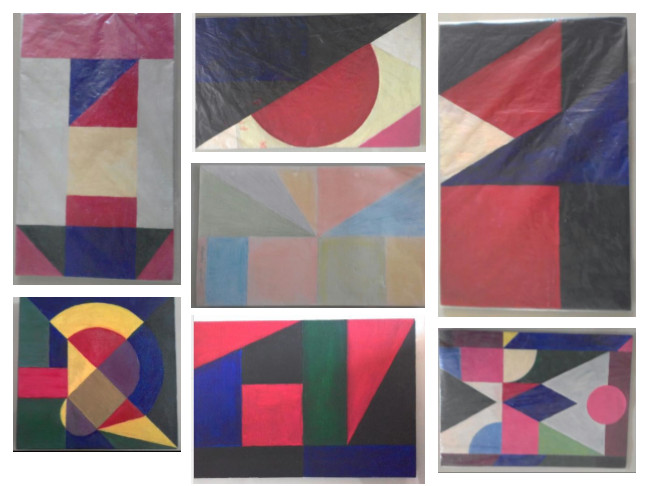
\includegraphics[width=.5\textwidth]{articles/04-matematica-na-arte--/figura1.jpg}%
        \caption*{Fonte: Elaborado pelo autor.}%
        \label{fig:figuras-planas}%
    \end{figure}%

    Vale ressaltar também que esta pesquisa foi realizada em uma Escola Pública da Rede Estadual do RN, em oito encontros vivenciais com duas turmas do 6º ano do Ensino Fundamental. Para esses encontros chamamos de “momentos”. Durante os encontros utilizamos como instrumento de coleta de dados, o diário de campo, para anotar nossas observações e as atividades práticas realizadas pelos alunos. A descrição de cada um desses “momentos” foi realizada em ordem cronológica para proporcionar uma melhor visão da pesquisa.  

    No primeiro momento apresentamos fotografias ampliadas de pinturas de autoria dos artistas Mondrian e Kandinsky conhecidos internacionalmente por utilizarem, em diversas de suas composições, elementos geométricos das mais variadas formas, conforme apresentadas nas Figuras \ref{fig:composicaoII}, \ref{fig:composition-a}, \ref{fig:arch-and-point} e \ref{fig:arch-and-point}. O nosso intuito foi tentar instigar o interesse dos alunos pelas figuras geométricas identificadas nas obras e, a partir de então, iniciar uma primeira discussão sobre como a Matemática interage com outras áreas do conhecimento, especialmente com a Arte. Neste momento discorremos sobre os conceitos elementares da Geometria, sobre figuras planas e suas principais propriedades. Percebemos que os estudantes tinham dificuldades em distinguir o círculo da circunferência, como também, em relação à ideia de raio e diâmetro. 

    \begin{figure}[ht]%
        \centering%
        \caption{Piet Mondrian, \textit{Composição II em Vermelho, Azul e Amarelo.}}%
        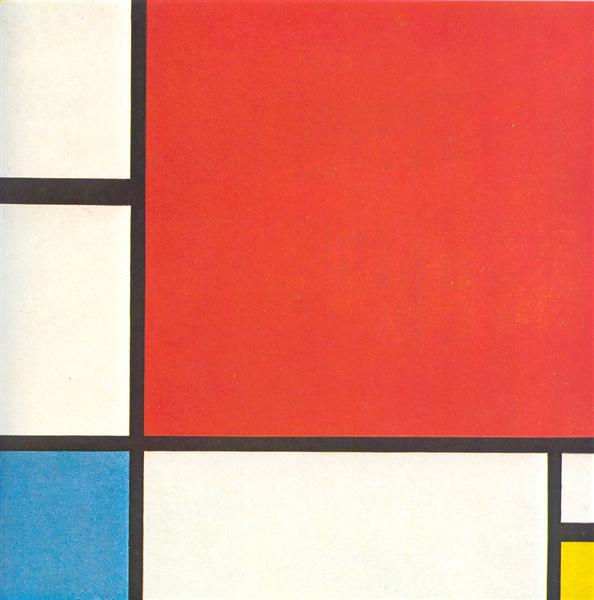
\includegraphics[width=.5\textwidth]{articles/04-matematica-na-arte--/figura2.jpeg}%
        \caption*{Fonte: \url{http://cultura.culturamix.com/arte/obras-de-piet-mondrian}}%
        \label{fig:composicaoII}%
    \end{figure}%
    
    \begin{figure}[ht]%
        \centering%
        \caption{Piet Mondrian, \textit{Composition A.}}%
        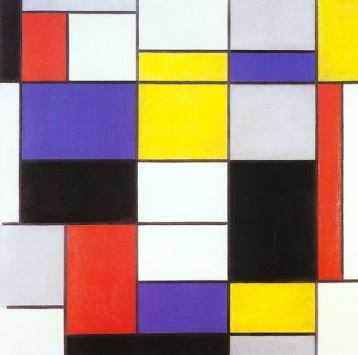
\includegraphics[width=.5\textwidth]{articles/04-matematica-na-arte--/figura3.jpeg}%
        \caption*{Fonte: \url{http://cultura.culturamix.com/arte/obras-de-piet-mondrian}}%
        \label{fig:composition-a}%
    \end{figure}%


    \begin{figure}[ht]%
        \centering%
        \caption{Wassily Kandinsky, \textit{Arch and Point.}}%
        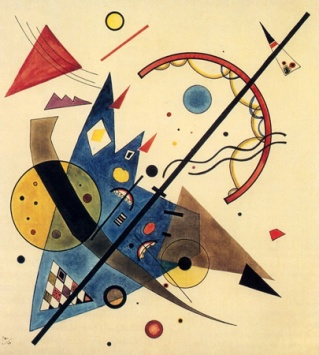
\includegraphics[width=.5\textwidth]{articles/04-matematica-na-arte--/figura4.jpeg}%
        \caption*{Fonte: \url{https://www.todocuadros.es/pintores-famosos/kandinsky/}}%
        \label{fig:arch-and-point}%
    \end{figure}%

    \begin{figure}[ht]%
        \centering%
        \caption{Wassily Kandinsky, \textit{On the points.}}%
        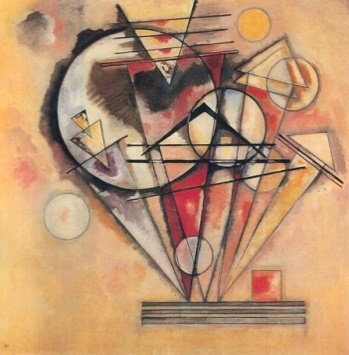
\includegraphics[width=.5\textwidth]{articles/04-matematica-na-arte--/figura5.jpeg}%
        \caption*{Fonte: \url{https://www.todocuadros.es/pintores-famosos/kandinsky/}}%
        \label{fig:on-the-point}%
    \end{figure}%

    No segundo momento iniciamos a aula expositiva com uma breve retomada. Nesta atividade objetivamos estimular a percepção visual por meio de cores e formas, bem como desenvolver o raciocínio a partir da prática da comparação, análise, identificação e a classificação das figuras planas presentes na tela em questão.  

    Apresentamos aqui as transcrições de alguns comentários dos alunos durante a realização da prática: “Eu nunca fiz tarefas de matemática utilizando telas de pintura ou figuras e, pensei que isso seria difícil”; “Não consigo formar novas figuras geométricas, pois elas já estavam todas formadas”; “Professor, não estou conseguindo mais me lembrar dos quadriláteros que estudamos na aula passada”; “Vai ser difícil, pois não sou artista”.  

    Dessa forma, na continuidade das atividades, realizamos algumas perguntas pertinentes ao conteúdo de Geometria, para gerar um debate, e assim surgirem as problemáticas a serem investigadas, entre elas, temos: O que é um quadrilátero? Quais os quadriláteros por nós estudados? O que diferencia um quadrado de um retângulo? Como são classificados os triângulos quanto aos lados? E, após essa breve discussão, novas dúvidas foram geradas e outras minimizadas, e aquela hesitação inicial diante da tarefa apresentada deu lugar à autoconfiança, que proporcionou uma mudança de atitude na qual propiciou a retomada da atividade proposta, como bem mostra a Figura \ref{fig:aluno-durante-pratica}.

    \begin{figure}[ht]%
        \centering%
        \caption{Aluno durante a prática da primeira atividade}%
        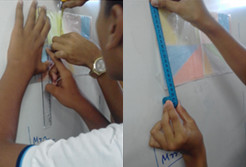
\includegraphics[width=.6\textwidth]{articles/04-matematica-na-arte--/figura6.jpg}%
        \caption*{Fonte: Elaborado pelo autor}%
        \label{fig:aluno-durante-pratica}%
    \end{figure}%

    O terceiro momento foi iniciado com um debate objetivando desenvolver a capacidade de observação e comparação entre os objetos e formas presentes no cotidiano dos alunos, mostrando a intensa presença da Matemática no mundo em que vivemos bem como, o quanto a Geometria apresenta-se envolvida ao nosso entorno, assim como despertar nos alunos o senso crítico para refletirem sobre como os artistas plásticos poderiam se beneficiar dos conhecimentos geométricos quando do desempenho de suas atividades profissionais.  

    Em seguida, apresentamos a atividade que teria como base as seis telas pintadas a óleo e elaboradas pelo pesquisador. Nessa atividade pedimos que os grupos identificassem as figuras planas presente nas obras e medissem o seu perímetro, como exemplificado na Figura \ref{fig:alunos-durante-2a-pratica}.

    \begin{figure}[ht]%
        \centering%
        \caption{Alunos durante a prática da segunda atividade}%
        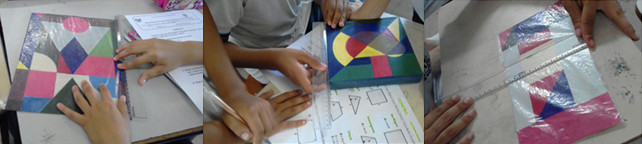
\includegraphics[width=.90\textwidth]{articles/04-matematica-na-arte--/figura7.jpg}%
        \caption*{Fonte: Elaborado pelo autor}%
        \label{fig:alunos-durante-2a-pratica}%
    \end{figure}%

    No quarto momento continuamos o estudo apresentando os conceitos de ângulos internos e de como medi-los por meio de um transferidor, bem como aferir dimensões utilizando régua, trena e fita métrica. Além de ensiná-los como proceder para executar os cálculos de área e de perímetro das principais figuras planas estudadas. Vale salientar que neste encontro utilizamos novamente as composições de Mondrian e Kandinsky com o propósito de justificar a importância dos conhecimentos geométricos para o processo criativo de tais pintores, além de proporcionar um momento de reflexão a respeito de como a Arte pode interagir com a Matemática e, no caso particular, com a Geometria.  

    Como essa forma de desenvolver os conteúdos causou um pouco de estranheza aos discentes, eles conseguiram assimilar bem nossa proposta e percebemos que nas turmas investigadas, no que se refere à desenvoltura apresentada ao longo das discussões, consideramos que o resultado foi bastante satisfatório, visto que emergiram consideráveis reflexões ao longo do debate. E esse fato deve ser levado em consideração, uma vez que estávamos lidando com alunos do 6º ano, recém-chegados às séries do Ensino Fundamental, anos finais, que tem uma estrutura de tempo e espaço diferente dos anos iniciais. 

    Quanto ao desempenho dos investigados durante a realização das atividades, constatamos que a proposta propiciou o desenvolvimento satisfatório da compreensão acerca das figuras geométricas e de suas aplicações no cotidiano das pessoas. Salientamos que, quanto à aferição de medidas de ângulos por meio do uso do transferidor, verificamos certa dificuldade que poderia ser justificada pelo fato de os alunos desconhecerem, até aquele momento, o referido instrumento de medida, bem como utilizá-lo. 

    No quinto momento, após a realização de algumas atividades práticas de verificação de medidas, utilizando-se de fita métrica, transferidor, trena e régua. Solicitamos que utilizassem o espaço da sala de aula e dos objetos, além das obras para realizar novas medições e fazer o cálculo de áreas, perímetro e ângulos. 

    Percebemos uma boa evolução no que diz respeito à interação e ao senso de cooperação dos alunos, visto que a resistência de alguns alunos de interagir com a sua equipe durante execução da atividade havia diminuído sensivelmente. Constatamos também, que a dificuldade apresentada, em momentos anteriores, para se verificar a medida de um ângulo interno de uma figura plana, utilizando o transferidor, já não existia. A Figura \ref{fig:alunos-durante-3a-pratica} nos dá uma breve noção do exposto anteriormente. 

    \begin{figure}[ht]%
        \centering%
        \caption{Alunos durante a prática da terceira atividade}%
        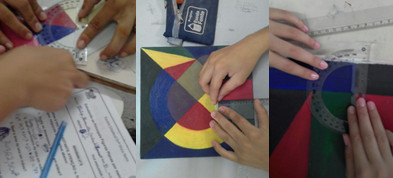
\includegraphics[width=.80\textwidth]{articles/04-matematica-na-arte--/figura8.jpg}%
        \caption*{Fonte: Elaborado pelo autor}%
        \label{fig:alunos-durante-3a-pratica}%
    \end{figure}%

    No sexto momento abrimos espaço aos alunos para que eles avaliassem a atividade realizada na aula anterior. A discussão foi bastante interessante, pois os investigados tiveram oportunidade de refletir sobre a importância de conhecer os conceitos geométricos referentes às figuras planas e, também, de como a utilização desse conhecimento poderia ser útil para a realização de diversas atividades do nosso dia a dia. Tudo isso, despertou o interesse dos alunos em tentar relacionar aqueles conteúdos estudados com a realidade de cada um.  

    Apresentamos aqui seis comentários proferidos pelos alunos: “Foi bom aprender como se medir usando a fita métrica e a trena”; “Saber calcular área e perímetro é importante para um engenheiro”; “Foi legal aprender como se usa um transferidor”; “Gostei muito de trabalhar usando uma fita métrica”; “Algumas coisas que a gente tem em casa podem ser medidas com uma trena”; “Saber usar uma trena é muito importante quando se quer verificar as medidas de um terreno ou de uma parede”. 

    A discussão realizada propiciou a retomada dos conteúdos apresentados ao longo dos encontros anteriores proporcionando o aprofundamento do debate em torno da aplicação dos conhecimentos de Geometria no dia a dia das pessoas bem como na área profissional, além disso, viabilizou um momento para que todos os participantes do estudo estabelecessem conexões entre os conteúdos apresentados em sala e os diversos ramos do conhecimento.  

    Por meio dessa ação os alunos observados tiveram a oportunidade de perceber a Geometria como uma ferramenta presente além dos muros da escola. Outro ponto a ser destacado desse momento diz respeito à possibilidade dada aos alunos de vislumbrarem o relevante papel que a Geometria desempenha na vida cotidiana do ser humano podendo ser considerada como ferramenta fundamental no processo de interação do indivíduo com o seu meio. Vale salientar que os conhecimentos inerentes à Geometria, além de constituírem a parte intuitiva da disciplina de Matemática, eles estão intimamente ligados à realidade das pessoas. 

    Após a realização do debate, propusemos uma rápida atividade prática de medição, como retratada na Figura \ref{fig:alunos-durante-6a-pratica}. Nessa atividade todos os grupos deveriam medir as dimensões da janela e da porta existentes na sala de aula usando como ferramenta de aferição uma trena ou uma fita métrica e, em seguida, realizariam o cálculo do perímetro e da área das referidas esquadrias.  

    \begin{figure}[ht]%
        \centering%
        \caption{Alunos durante a prática no sexto momento da pesquisa}%
        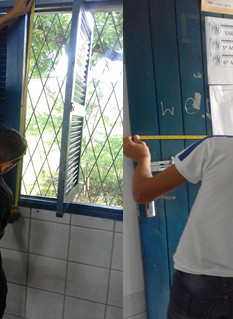
\includegraphics[width=.25\textwidth]{articles/04-matematica-na-arte--/figura9.jpg}%
        \caption*{Fonte: Elaborado pelo autor}%
        \label{fig:alunos-durante-6a-pratica}%
    \end{figure}%

    Essa atividade foi interessante, uma vez que os grupos tiveram a oportunidade de verificar que, devido a pequenas diferenças no que diz respeito ao trabalho de aferição das dimensões da janela e da porta, os valores calculados para o perímetro e para a área não foram exatamente iguais entre os respectivos grupos, apresentavam algumas diferenças de aproximadamente entre um centímetro a dois centímetros, mas nada que preocupasse tanto, pois entendemos que nossos instrumentos de medidas são rudimentares e o seu manuseio pode levar a pequenas diferenças de medidas. 

    Mas, isso nos deu a oportunidade de evidenciar para os alunos participantes da investigação da importância de executar uma aferição cuidadosa, uma vez que, ao aferirmos erroneamente uma determinada medida, iremos comprometer os resultados finais do nosso trabalho, e pode também nos levar a perda de materiais, caso fizéssemos uma maquete para representar nossos estudos de sala de aula. 

    Já no sétimo momento, tínhamos por objetivo estimular o viés artístico de cada um dos alunos, pois na referida atividade, constava uma questão que solicitava a composição de um desenho no qual o tema seria figuras planas. E ainda, solicitamos que observassem os ambientes fora da escola e anotassem os objetos identificados e associados com as figuras geométricas. 

    De início, realizamos uma discussão a respeito da presença de elementos geométricos no nosso cotidiano. Listamos, a critério de elucidação positiva dos momentos vivenciados ao longo do processo, oito comentários dos alunos: “Eu vejo figuras planas em muitos prédios”; “A geometria está presente em praças e calçadas da cidade”; “As portas, janelas e portões das casas têm forma de retângulos e quadrados que são figuras planas”; “Têm muitas figuras geométricas em minha casa”; “Muitas coisas que encontramos na rua, possuem as formas geométricas que aprendemos aqui nessas aulas”; “As formas geométricas estão presentes nos azulejos das paredes da cozinha de minha casa”; “As placas de trânsito têm as formas de triângulo, de quadrado e de círculo”; “Muitos artistas utilizam os conhecimentos de Geometria para fazer suas telas”. 

    E, no nosso oitavo momento foi realizado um debate rico pela troca de experiências vivenciadas e de reflexão a respeito das novas descobertas. Eis aqui em destaque oito comentários proferidos pelos alunos: “Essa última atividade foi boa porque a gente viu as figuras planas em muitos prédios”; “Achei legal essa atividade porque aprendemos a fazer desenhos, usando muitas figuras planas do jeito que os artistas famosos fazem”; “Gostei dessa atividade porque aprendi sobre a importância das figuras planas para os engenheiros”; “As figuras planas estão em muitos objetos de nossas casas”; “Gostei de saber como é importante usar corretamente uma trena”; “Estudar figuras planas foi importante porque a Geometria está presente na nossa vida”; “Esta atividade foi legal porque vimos na prática como os artistas podem utilizar os conhecimentos de geometria para realizar as suas obras”; “Gostei de saber que até nas Artes têm Matemática”.  

    Realizamos uma culminância das atividades desenvolvidas, assim oportunizamos os grupos a apresentarem as suas composições, colocamos a representação de algumas delas na Figura \ref{fig:composicoes-3-grupos}. 

    \begin{figure}[ht]%
        \centering%
        \caption{Composições elaboradas por três dos grupos participantes.}%
        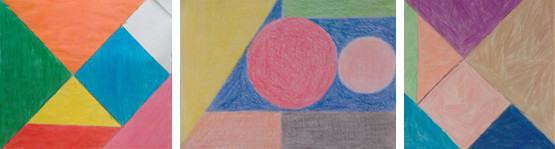
\includegraphics[width=.90\textwidth]{articles/04-matematica-na-arte--/figura10.jpg}%
        \caption*{Fonte: Elaborado pelo autor}%
        \label{fig:composicoes-3-grupos}%
    \end{figure}%

    \section{Considerações finais}

    A análise do processo desenvolvido evidenciou como a Arte pode contribuir no ensino e aprendizagem de Geometria. Uma vez que a utilização de pinturas em sala foi satisfatória, visto que o procedimento promoveu o interesse do aluno pela discussão em torno da importância dos conhecimentos geométricos para outras áreas do conhecimento. Percebemos também que, a utilização de telas de pintores renomados nas aulas, proporcionou ao aluno uma modificação do seu olhar no que diz respeito à importância da Geometria para o desempenho de muitas atividades do nosso cotidiano, tais como: a aferição de medidas de dimensão, o cálculo de áreas e de perímetros, dentre outros saberes.  

    Com esta proposta, também foi dada a oportunidade de se discutir, por exemplo, como o conhecimento geométrico pode ser útil para um artista durante o processo de composição de uma obra, propiciando assim, um pensar sobre a Geometria como algo de grande utilidade presente na nossa vida. 

    Os resultados advindos desta pesquisa mostram que, ao longo de todo o processo, os alunos apresentaram alterações, tanto no interesse quanto na participação, pois foi percebida uma mudança positiva de atitude, principalmente, daqueles que apresentavam um comportamento menos participativo em nossas aulas. Isso, pois, durante as atividades os alunos manifestaram seus questionamentos, ideias e reflexões a respeito das possibilidades de utilização dos conceitos geométricos referentes às figuras planas no nosso cotidiano.   

    Outro ponto a ser destacado diz respeito à Arte como facilitadora do processo ensino e aprendizagem, visto que, devido ao seu viés estético e lúdico o recurso da Arte mostrou-se como valioso elemento para o ensino da Geometria como também para a construção do saber de cada um dos envolvidos no processo, pois ao dar oportunidade de manusearem diferentes instrumentos de medidas, propiciou a construção de um ambiente de discussão no qual contribuiu tanto para a ampliação dos conhecimentos quanto para desenvolvimento da habilidade de expressar opinião, ou seja, de argumentação, como também desenvolveu, em cada um dos envolvidos, as habilidades artísticas, visto que uma das atividades propostas aos investigados era a criação de uma obra a ser realizada em grupo e cujo tema girava em torno das figuras geométricas estudadas durante o processo.  

    Não identificamos limitações para a utilização da Arte como caminho para o ensino e aprendizagem da Matemática. Percebemos que as aprendizagens apresentaram bons resultados, quanto a assimilação dos conteúdos, e apontamos que isso aconteceu devido a forma com que foram desenvolvidas as atividades, por meio da experimentação, e utilizando a observação e o contato com as formas geométricas, além de poderem ter tido a oportunidades de utilizar alguns instrumentos medidas tanto para verificar as figuras dos quadros como para se inspirarem e produzirem suas pinturas autorais. 

    Esperamos que esse artigo sirva de inspiração para todos aqueles profissionais que trabalham com educação de jovens em um contexto similar ao investigado nessa pesquisa e que desejam utilizar a Arte como uma possível aliada ao ensino da Matemática, em especial, ao Ensino da Geometria, pois, mesmo que não sejamos profundos conhecedores dessa área de conhecimento, todos nós temos plenas condições de propiciar algo de relevância que nos possibilite viabilizar relações significantes entre a área da Arte e da Matemática, e que sejam capazes de contribuir na apropriação de novos conceitos e demandas surgidas durante o processo de ensino e aprendizagem da Matemática, e em especial, a Geometria. 

    \printbibliography[heading=subbibliography,notcategory=fullcited]

    \label{chap:matematicanaarteend}

\end{refsection}
